\clearpage\section{Research lineage: lifecycle security to evidence-grounded AI}
The research programme underlying this collection began in 2023 with \textit{Digital Twins and the Future of Their Use Enabling Shift Left and Shift Right Cybersecurity Operations}, by Mohsin, Janicke, Nepal and Holmes [15]. Its September 2023 preprint and TPS-ISA 2023 record establish this starting point. The work placed security digital twins across the CPS lifecycle: \emph{shift left} brings security analysis into design, while \emph{shift right} supports analysis during operation. This history concerns the research programme; it does not imply that every released data record was collected in 2023.

\subsection*{From lifecycle models to interpretable security analysis}
The subsequent state-of-the-art AI/XAI review by Sarker, Janicke, Mohsin, Gill and Maglaras [16] organized AI and explainable-AI methods for cybersecurity in digital-twin environments. It provides a methodological foundation for examining the quality and interpretability of security analytics. The later chapter \textit{Security risks and privacy challenges in digital twins} [17] extended the lifecycle perspective to security, privacy and architectural concerns, including a smart-factory case study.

LLM-enabled reasoning represents a later strand of this programme rather than a capability that should be attributed retrospectively to every earlier publication. The guide's graph-grounded CTI and query-generation studies connect to NeuroGraph [2]; its separation of recommendations from permission to act also relates to the trusted-autonomy work [3]. BRIDG-ICS [1] and HySecTwin [4] provide further context for graph integration and hybrid reasoning. These connections motivate the research questions; they do not establish that the public subset reproduces each article's experiments.

\subsection*{Sector-specific modelling and the present research resource}
The railway paper, \textit{A Secure-by-Design Virtual Twin Framework for AI-Driven Threat Modeling in Railway OT Systems} [18], places virtual-twin threat modelling in a transport-OT setting. It is included as a related sector-specific work. Railway records are not asserted to be present in this industrial dataset, and transfer of a method requires the independent validation described in the cross-sector study.

\begingroup\small\renewcommand{\arraystretch}{1.25}
\begin{tabularx}{\linewidth}{>{\raggedright\arraybackslash}p{28mm}>{\raggedright\arraybackslash}X>{\raggedright\arraybackslash}X}
\toprule
\textbf{Research strand} & \textbf{Prior-work connection} & \textbf{Use in this guide}\\\midrule
Lifecycle security & Shift-left/shift-right digital twins [15] & Design-stage topology studies and operational monitoring questions\\
Interpretable analytics & AI/XAI methods and taxonomy [16] & Baseline comparisons, explanation support and error analysis\\
Security and privacy & Digital-twin lifecycle and architecture [17] & Provenance, pseudonymization and evidence limitations\\
LLMs and reasoning & NeuroGraph and trusted autonomy [2,3] & Grounded answers, semantic queries and bounded decisions\\
Sector application & Railway virtual-twin work [18] & Transfer questions and sector-specific validation requirements\\
\bottomrule\end{tabularx}\endgroup

The present collection makes selected representations and offline fixtures available for further investigation of these themes. Its value lies in enabling transparent, bounded experiments across structural, synthetic, observational and expected-decision evidence. Researchers should cite the relevant intellectual foundations as well as this particular dataset release.

\clearpage\section{Intellectual development and research positioning}
The following schematic traces related research themes. Arrows indicate conceptual development, not a claim that each publication used the present public subset or that its experiments are reproducible from this collection alone.

\begin{center}
\begin{tikzpicture}[node distance=9mm]
\node[block,design,text width=128mm] (origin) {\textbf{2023: lifecycle security foundations [15]}\\Shift-left design analysis and shift-right operational security};
\node[block,input,text width=128mm,below=of origin] (review) {\textbf{2024: AI and explainable-AI review [16]}\\Methods, taxonomy, interpretability and trustworthiness};
\node[block,method,text width=128mm,below=of review] (extension) {\textbf{Subsequent research strands [1--4,17,18]}\\Hybrid reasoning and graph-grounded LLMs\\Trusted autonomy, security/privacy and railway virtual twins};
\node[block,evaluation,text width=128mm,below=of extension] (resource) {\textbf{Present public research collection}\\Structural, synthetic, observational and expected-decision evidence};
\node[block,output,text width=128mm,below=of resource] (studies) {\textbf{Further independently evaluated studies}\\Declared hypotheses, held-out groups, baselines and bounded claims};
\draw[arr](origin)--(review);\draw[arr](review)--(extension);\draw[arr](extension)--(resource);\draw[arr](resource)--(studies);
\end{tikzpicture}
\end{center}
\textbf{How to cite the connection.} Cite the 2023 work when discussing lifecycle security, the review when discussing AI/XAI methods, and the relevant later article when adopting its method. Cite the dataset version for the specific public inputs used. Intellectual lineage and empirical provenance serve different purposes.

\textbf{What this resource adds.} The collection assembles selected representations and fixtures with provenance, component licensing and reproducibility guidance. Demonstrating a new security capability requires a separately specified experiment. In particular, neither architectural relevance nor a related publication supplies missing incident labels or physical validation.

\clearpage\section{Research question--data--evaluation matrix}
Each question must be evaluated at the level supported by its evidence. An editable companion matrix is available in the repository at\newline \texttt{docs/RESEARCH\_QUESTIONS.md}.

\begingroup\footnotesize\renewcommand{\arraystretch}{1.32}
\begin{tabularx}{\linewidth}{>{\raggedright\arraybackslash}p{31mm}>{\raggedright\arraybackslash}X>{\raggedright\arraybackslash}X}
\toprule\textbf{Question and inputs} & \textbf{Method and evaluation} & \textbf{Suitability and limit}\\\midrule
Monitoring allocation: inventory and flows & Boundary-aware versus degree-based placement; weighted coverage at fixed cost & Structural comparison; service-loss reduction unmeasured\\
CWE prediction: graph mappings & Typed model versus training-label popularity; whole-CVE holdout; Hit@k and MRR & Upstream mapping recovery; remove target/inverse edges\\
Grounded CTI: benchmarks and graph & Retrieval versus no retrieval; grouped descriptions; exact match, unsupported identifiers and coverage & Requires overlap audit and controlled model settings\\
Event novelty: operational traces & Rarity versus transitions; whole-trace holdout; flag and unseen-class rates & Exploratory; verified attack labels absent\\
Query generalization: training pairs & Base versus adapted model; new template-disjoint test set; semantic agreement & New evaluation set required\\
Decision governance: agent fixtures & Guarded versus unguarded policy; family holdout; class recall and prohibited-decision rate & Expected-decision agreement; no physical safety inference\\
Evidence robustness: derived variants & Clean versus declared perturbations; paired decision-change rates & New perturbation protocol required\\
Analyst triage: verified evidence joins & Controlled study; task accuracy, review time and confidence calibration & New participant evidence and valid joins required\\
\bottomrule\end{tabularx}\endgroup

\textbf{Reporting standard.} State the independent evaluation unit, exclusion rules, fixed partitions, baseline and uncertainty. Fit thresholds and preprocessing on training groups. Report failures and abstentions. For graph methods, document candidate labels and all retained relation paths. For temporal data, avoid treating dependent rows as independent replicates.

\clearpage\section{Runnable starter protocols and measured baselines}
The new examples use only Python's standard library. From the repository root, run:
\begin{Verbatim}[fontsize=\small,breaklines=true]
python3 examples/run_starters.py --output /tmp/cps-starters
python3 examples/check_starters.py
\end{Verbatim}
The checked-in results and split manifest are under \texttt{examples/baselines}. These newly introduced illustrative partitions are not official benchmark splits or reproductions of the cited articles.

\begingroup\small\renewcommand{\arraystretch}{1.3}
\begin{tabularx}{\linewidth}{>{\raggedright\arraybackslash}p{29mm}>{\raggedright\arraybackslash}X>{\raggedright\arraybackslash}X}
\toprule\textbf{Starter} & \textbf{Protocol} & \textbf{Measured reference result}\\\midrule
Event rarity & Train-only event frequencies and 95th-percentile threshold; 21 training and 6 test traces & 420 test events; 2.38\% flagged; 0.95\% unseen event classes\\
CWE popularity & Training-only CWE frequency; whole-CVE hash split; 44,188 test CVEs & Hit@1: 0.1676; Hit@5: 0.4038; MRR: 0.2868\\
Constant-stop decision & Four held-out scenario families; 60 test cases with explicit boolean stop expectations & Agreement: 0.6667; continue recall: 0; 220 cases without boolean stop excluded across all families\\
\bottomrule\end{tabularx}\endgroup

\textbf{Split design.} Operational and graph groups use SHA256 of a versioned group key modulo five. The agent test families are SC-02, SC-06, SC-14 and SC-18; this explicit selection includes both decision classes. Family selection was made when introducing the protocol. Freeze these groups for subsequent comparisons; independently authored families remain desirable because scenario families may share rules.

\textbf{Interpretation.} Rarity flags are not malicious-event detections. CWE scores measure agreement with source-reference mappings. The constant-stop baseline illustrates why overall agreement should be accompanied by class-specific results. Missing expected fields are not inferred. No physical system, live model or attack tool is executed.

\textbf{Trace interpretation.} The 14,124 events contain 27 distinct trace identifiers. Reproducibility checks cover group assignment, class coverage, recorded results and repeated execution. Trace-level metadata supports explicit eligibility rules for sequence studies.

\textbf{Versioned citation.} Cite the tagged release and applicable upstream works. The existing \texttt{CITATION.cff} provides citation metadata. Use the repository version or commit identifier to identify the exact files used. The archival guide explains persistent citation options.


\clearpage\section{Contemporary security problems, 2025-2026}
\subsection*{Loss of monitoring and control through exposed PLCs}
A July 2026 FBI/EPA announcement reports water-sector incidents involving internet-facing PLCs, with changes to configurations and credentials causing loss of monitoring or control [9]. This motivates research on communication boundaries, trusted configuration evidence and restoration priorities. The inventory and graph tables support an abstract comparison of exposure-reduction policies; they contain neither packet captures nor forensic records of those incidents.

\subsection*{Authority and reliability in AI-enabled OT}
The December 2025 joint guidance on secure AI integration in OT emphasizes suitability assessment, governance, oversight and lifecycle testing [10]. A research implication is that model accuracy and permission to act should be evaluated separately. The agent fixtures can test tool eligibility and stop decisions. Their expected outputs cannot establish the safety of direct process control.

\subsection*{Manipulated inputs and ungrounded explanations}
NIST 2025 adversarial machine-learning taxonomy covers attacks across the AI lifecycle [11]. For this corpus, a tractable research question concerns whether controlled corruption of graph facts or retrieved evidence changes an analytical conclusion. Such experiments require newly constructed perturbations with explicit attacker capabilities; the release does not supply a validated poisoning or prompt-injection benchmark.

\textbf{Sources:} [9] FBI/EPA, 30 July 2026: \href{https://www.fbi.gov/investigate/cyber/alerts/2026/malicious-cyber-actors-targeting-water-and-wastewater-sector-internet--facing-programmable-logic-controllers-causing-operational-disruptions}{Water-sector PLC warning}. [10] ASD and international partners, 4 December 2025: \href{https://www.cyber.gov.au/publication/principles-for-the-secure-integration-of-artificial-intelligence-in-operational-technology}{Secure AI integration in OT}. [11] Vassilev et al., March 2025: \href{https://doi.org/10.6028/NIST.AI.100-2e2025}{NIST AI 100-2 E2025}. 

These connections are proposed research uses, not claims that the dataset contains contemporary campaigns. The security contribution should be stated at the level actually evaluated: topology, reference mapping, controlled robustness or fixture-level decision behavior.

\clearpage\section{Potential research areas and open problems}
\begingroup\small\setlength{\tabcolsep}{5pt}\renewcommand{\arraystretch}{1.22}
\begin{tabularx}{\linewidth}{>{\raggedright\arraybackslash}X>{\raggedright\arraybackslash}X>{\raggedright\arraybackslash}X}
\toprule
\textbf{Area / open problem} & \textbf{Testable question} & \textbf{Inputs and expected contribution}\\
\midrule
Exposure and segmentation & Can boundary-aware monitoring improve weighted flow coverage at the same budget? & Inventory + topology; resource-allocation method\\
Explainable graph inference & Does relation typing improve held-out link ranking without inverse-edge leakage? & Knowledge graph; auditable structural inference\\
Grounded CTI analytics & Does graph evidence reduce unsupported identifiers at matched answer coverage? & CTI benchmarks + graph; calibrated mapping\\
Security query generation & Does adaptation generalize beyond familiar query templates? & Training pairs + new disjoint test set; semantic validation\\
Behavioral anomaly analysis & Can unusual transitions be detected across held-out traces? & Operational traces; exploratory or adjudicated evaluation\\
Adversarial AI robustness & How much controlled evidence corruption changes a decision? & Derived graph/CTI variants; robustness characterization\\
Agent governance & Do policy guards reduce prohibited decisions under held-out scenario families? & Expected-decision fixtures; explicit policy evaluation\\
Human-centered triage & Does a traceable evidence chain improve reviewer accuracy and review time? & Validated joins + new analyst study; decision-support evaluation\\
\bottomrule\end{tabularx}\endgroup\par\medskip
The interpretability questions are informed by the earlier AI/XAI review [16]. The questions are deliberately comparative. A new model name or higher score alone is insufficient: the experiment should isolate the proposed mechanism, define the independent evaluation unit and identify the practical meaning of the observed difference. No novelty claim is implied without a separate literature review.

\clearpage\section{Dataset suitability and evidence gaps}
Suitability is assessed for a specified research claim rather than for an algorithm in isolation. Direct support means that the necessary released inputs exist for a bounded offline task. Conditional support means that labels, mappings or an evaluation set must be added. Unsupported claims require a different empirical basis.

\begingroup\small\setlength{\tabcolsep}{5pt}\renewcommand{\arraystretch}{1.22}
\begin{tabularx}{\linewidth}{>{\raggedright\arraybackslash}X>{\raggedright\arraybackslash}X>{\raggedright\arraybackslash}X}
\toprule
\textbf{Data family} & \textbf{Suitability in this release} & \textbf{Additional evidence for broader claims}\\
\midrule
Inventory & Direct: topology, boundary coverage and prioritization & Observed configurations, controls and exposure validation\\
Knowledge graph & Direct: typed relation analysis; conditional: risk inference & Adjudicated relations; time-stamped updates; measured outcomes\\
CTI benchmarks & Direct: reference-label mapping comparisons & Independent label review; evidence corpus for faithfulness\\
Training pairs & Conditional: adaptation and query generation & Template-disjoint held-out prompts; semantic oracle\\
Synthetic & Direct: controlled sensitivity experiments & Real incident labels and external operational validation\\
Operational & Direct: sequence description; conditional: intrusion detection & Attack/fault adjudication; signal meanings; physical context\\
Agent scenarios & Direct: expected-policy agreement & Actual execution traces; independent outcome and safety criteria\\
Cross-source fusion & Conditional: only validated joins & Identity/time mappings and a documented coverage audit\\
\bottomrule\end{tabularx}\endgroup\par\medskip
The corpus alone is unsuitable for measuring field intrusion-detection effectiveness, certifying autonomous control, estimating sector-wide attack prevalence, proving causal physical consequences, or establishing a current vulnerability risk score. These are evidence limitations, not conclusions about the usefulness of the data.

\clearpage\section{A focused study of adversarial AI robustness}
A defensible extension is to examine whether analytical outputs remain stable when a bounded portion of their evidence is manipulated. The independent variable is the perturbation budget; the primary outcome is the change in correctness or unsupported-claim rate relative to a clean evaluation. The threat model must specify access, knowledge and the records that an adversary can modify.

\begin{figure}[H]\centering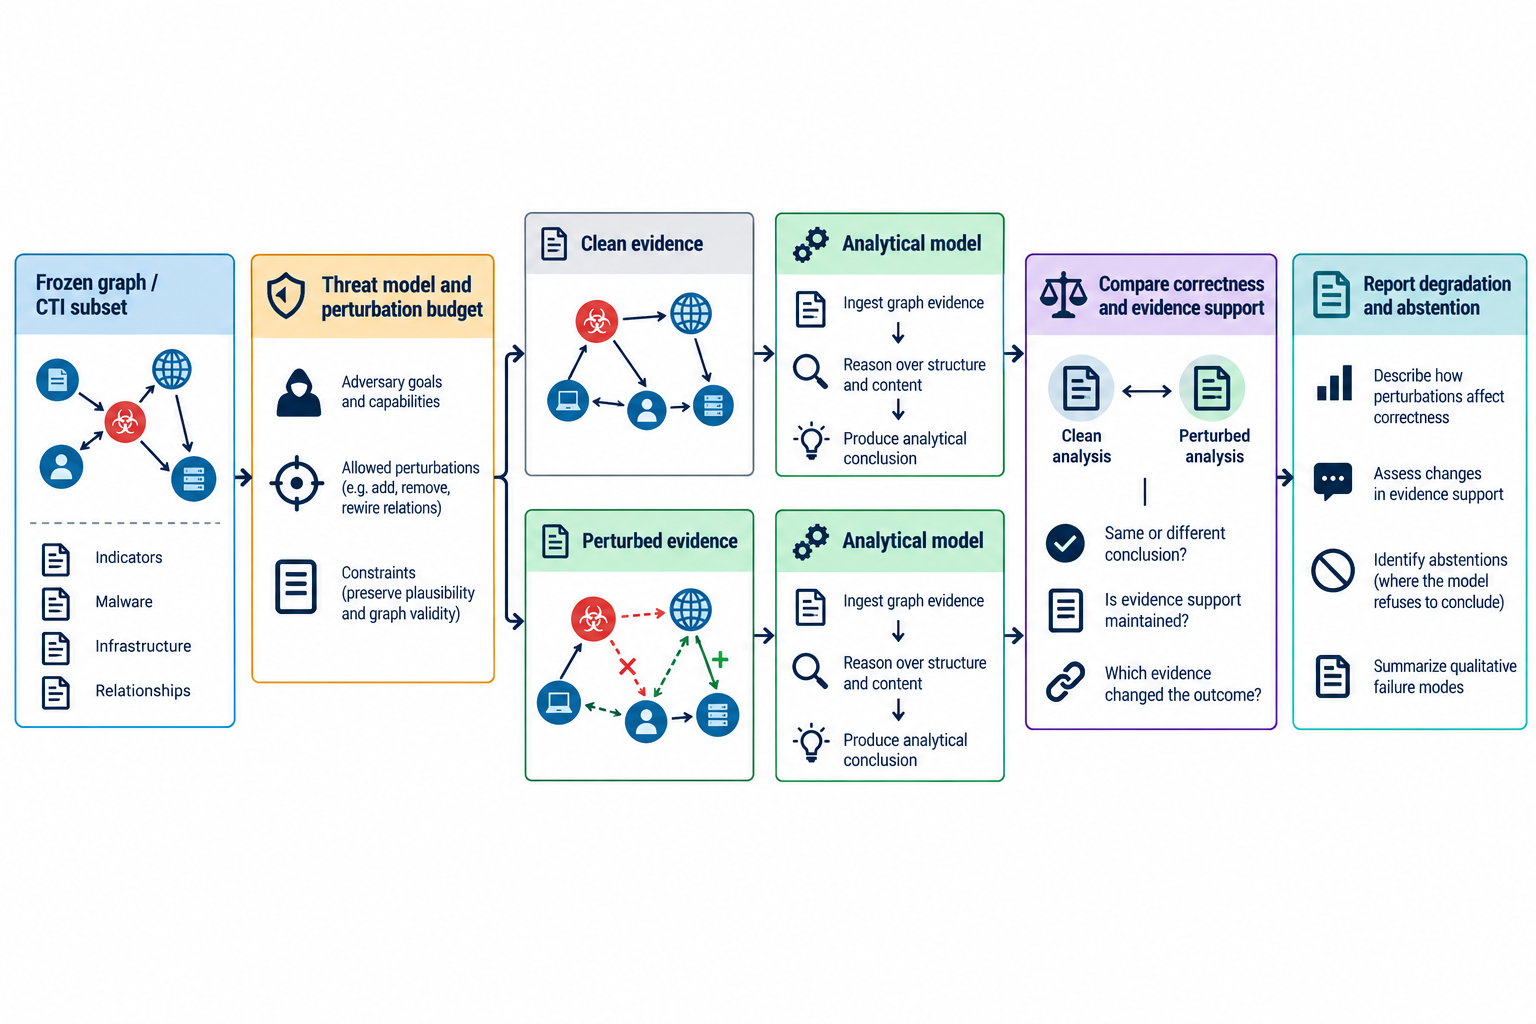
\includegraphics[width=\linewidth,trim={0bp 222bp 0bp 192bp},clip]{images/figure-04.png}\caption{Controlled evidence manipulation. Blue: evidence; amber: design; grey/green: comparison; purple: evaluation; teal: reporting.}
\end{figure}
Researchers may remove relations, introduce type-consistent false relations, or add conflicting retrieved statements to derived copies. Each variant should record affected IDs and its construction rule. Label leakage, malformed inputs and plausible but incorrect evidence should be analyzed separately. Prompt injection requires a separately constructed textual corpus and task-specific success criteria; no such benchmark is supplied.

Useful outcomes include degradation curves, false-evidence acceptance, abstention under contradiction and recovery after evidence removal. Results support a claim about the declared perturbation model, not about resistance to all adaptive adversaries.

\clearpage\section{Cross-sector relevance and transfer limits}
\begin{figure}[H]\centering
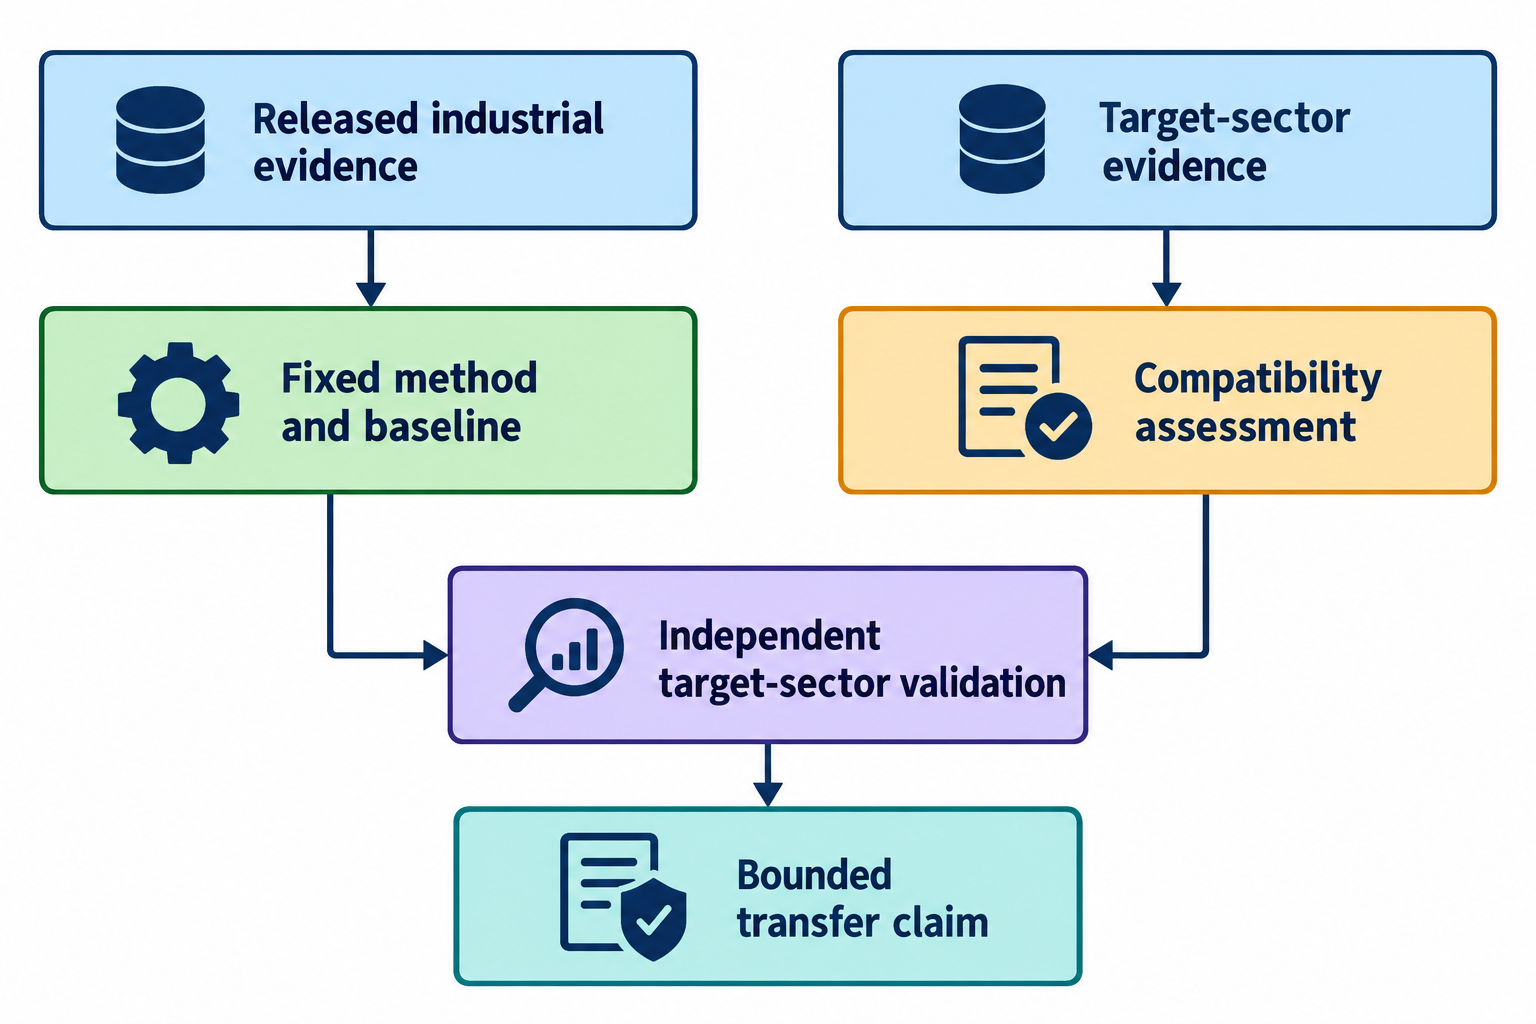
\includegraphics[width=\linewidth,trim={19bp 18bp 19bp 30bp},clip]{images/figure-05.png}\caption{Evidence required for cross-sector transfer. }\end{figure}
\begingroup\small\setlength{\tabcolsep}{5pt}\renewcommand{\arraystretch}{1.22}
\begin{tabularx}{\linewidth}{>{\raggedright\arraybackslash}X>{\raggedright\arraybackslash}X>{\raggedright\arraybackslash}X}
\toprule
\textbf{Application context} & \textbf{Transferable research method} & \textbf{Required sector-specific additions}\\
\midrule
Water and wastewater & Boundary analysis; change/anomaly triage & Hydraulic/process model, asset mapping, quality/pressure limits\\
Electricity and DER & Evidence-grounded prioritization; guarded recommendations & Electrical topology, grid dynamics, protection and timing constraints\\
Manufacturing & Flow coverage; sequence analysis; agent fixture evaluation & Verified station semantics, production modes and incident labels\\
Transport services & Dependency reasoning and evidence provenance & Relevant control systems, interlocks, operational and safety outcomes\\
\bottomrule\end{tabularx}\endgroup\par\medskip
Cross-sector applicability is a hypothesis to test. Similar network protocols do not imply equivalent dynamics, hazards or response authority. The transfer diagram identifies the additional evidence required to evaluate that hypothesis.

\clearpage\section{Threats to validity and research interpretation}
\subsection*{Construct validity}
A proxy must be distinguished from the phenomenon of interest. Coverage of declared flows measures monitoring placement, not prevention of compromise. Expected policy agreement measures consistency with an oracle, not physical safety. Unusual event sequences measure deviation, not necessarily malicious behavior.

\subsection*{Internal validity}
Duplicate descriptions, repeated attackability tables and inverse graph relations can contaminate a comparison. Preprocessing, retrieval indexing and hyperparameter selection must follow the split. For LLM studies, expected answers and direct answer-bearing records should be excluded from the evaluated input. Model pretraining contamination remains a separate uncertainty.

\subsection*{External validity}
The industrial setting, pseudonymization, synthetic assumptions and small number of independent traces restrict generalization. A large row count does not substitute for independent sites, operating modes or incidents. Transfer studies should evaluate an additional, independently curated dataset and disclose differences in sensors, protocols and labels.

\subsection*{Statistical conclusion validity}
Repeated windows from one trace are correlated. Confidence intervals should reflect grouping by trace, entity, description or scenario family. Multiple model comparisons should be distinguished from a prespecified primary analysis. Effect sizes and failure distributions are more informative than isolated best-run scores.

A manuscript should acknowledge these limitations where the relevant result is interpreted, rather than relying only on a general limitations paragraph.

\clearpage\section{Study protocol and figure conventions}
\subsection*{From research problem to an assessable claim}
The lifecycle framing follows the shift-left/shift-right research [15,17]. A study protocol should state the operational motivation, the hypothesized mechanism, the released evidence, the intervention or model variation, and the outcome that could refute the hypothesis. A primary endpoint and evaluation split should be frozen before tuning. The baseline should represent a credible simpler approach under the same information and resource budget.

For example: under a fixed monitoring budget, a boundary-aware policy is hypothesized to cover a larger weighted proportion of declared cross-zone flows than degree ranking. A negative or negligible difference would refute the proposed benefit for this topology. The conclusion would concern the declared graph, with no claim about measured attack reduction.

\subsection*{Consistent meaning of workflow colours}
\begingroup\small\setlength{\tabcolsep}{5pt}\renewcommand{\arraystretch}{1.22}
\begin{tabularx}{\linewidth}{>{\raggedright\arraybackslash}X>{\raggedright\arraybackslash}X}
\toprule
\textbf{Colour} & \textbf{Role in the experimental argument}\\
\midrule
Blue & Released evidence or frozen inputs\\
Amber & Study design, split construction or eligibility checks\\
Grey & Baseline or reference condition\\
Green & Proposed method or permitted branch\\
Coral & Held, rejected or unsupported branch\\
Purple & Common evaluation or evidence review\\
Teal & Reported outputs, uncertainty and provenance\\
\bottomrule\end{tabularx}\endgroup\par\medskip
Each box also states its role in text so the diagrams remain interpretable in greyscale. Comparison diagrams share inputs and evaluation conditions. Decision diagrams distinguish permitted and held branches. All workflows describe proposed research procedures, rather than newly measured experimental results.

The following sections document the evidence inventory, data loading, study protocols, evaluation measures and reproducibility requirements. Use the PDF bookmarks to navigate the guide.

\clearpage\section{Choose the evidence and the question}
\begingroup\small\setlength{\tabcolsep}{5pt}\renewcommand{\arraystretch}{1.22}
\begin{tabularx}{\linewidth}{>{\raggedright\arraybackslash}X>{\raggedright\arraybackslash}X>{\raggedright\arraybackslash}X}
\toprule
\textbf{Folder / evidence} & \textbf{Release size} & \textbf{Research use}\\
\midrule
inventory / structural tables & 94 master assets; 53 component records; 120 flows; 6 zones; 5 conduits & Segmentation and exposure\\
knowledge\_graph / typed structure & 305,167 nodes; 276,420 edges & Link prediction and graph reasoning\\
benchmarks / upstream reference labels & 2,047 CTI records & CTI extraction and mapping\\
training / instruction-output examples & 358 unique pairs & Query generation and adaptation\\
synthetic / generated assumptions and logs & 340 attackability rows; 9,880 protocol rows & Controlled perturbations\\
operational / pseudonymized observations & 14,124 events; 27 traces & Sequence and anomaly studies\\
agent\_scenarios / expected fixtures & 20 scenarios; 400 cases & Governed decision behavior\\
\bottomrule\end{tabularx}\endgroup\par\medskip
Folder counts are not independent evidence units. Some attackability tables are repeated in the graph and synthetic folders; do not count the same rows as independent replications.

\subsection*{Evidence classes matter}
An observed event is not automatically an attack. A synthetic risk score is an assumption, not a measured compromise probability. A reference answer is not a newly adjudicated label. An expected agent output is a test oracle, not a successful tool execution. Graph referential integrity is not semantic truth.

Read data/README.md, the selected folder README, docs/SCHEMAS.md, docs/DATASET\_CARD.md and metadata/licenses.csv before selecting features. Use metadata/provenance.csv and \path{metadata/research_file_map.csv} to trace inputs and related research.

\clearpage\section{Obtain, freeze and load the release}
\begin{Verbatim}[fontsize=\footnotesize,breaklines=true,frame=single,rulecolor=\color{rulegray},framesep=8pt]
git clone https://github.com/ahmadspm/industrial-cps-security-datasets.git
cd industrial-cps-security-datasets
git rev-parse HEAD
python scripts/validate_release.py
\end{Verbatim}
Record the full commit, Python version and file SHA-256 values from metadata/checksums.csv. Run the validator from the repository root. Work in a separate output directory and retain the original compressed inputs unchanged.

\subsection*{CSV and compressed CSV: standard-library loader}
\begin{Verbatim}[fontsize=\footnotesize,breaklines=true,frame=single,rulecolor=\color{rulegray},framesep=8pt]
from pathlib import Path
import csv, gzip, json

def rows(path):
    path = Path(path)
    opener = gzip.open if path.suffix == ".gz" else open
    with opener(path, "rt", encoding="utf-8-sig", newline="") as f:
        yield from csv.DictReader(f)

flows = list(rows("data/inventory/Dataflows.csv"))
cves = rows("data/knowledge_graph/cve_node_000.csv.gz")
first_cve = next(cves)
with gzip.open("data/operational/event_features.jsonl.gz",
               "rt", encoding="utf-8") as f:
    first_event = json.loads(next(f))
with open("data/training/fine_tuning.json", encoding="utf-8") as f:
    instruction_pairs = json.load(f)
\end{Verbatim}
CSV values load as strings. Convert numeric and boolean columns explicitly from the schema; distinguish missing values from zero. Stream all 15 CVE shards for the full CVE table. Do not load a plain CSV sibling in addition to its compressed release file.

No database service is needed to inspect the data. A graph store, embedding model or LLM is a researcher-selected addition and must be versioned separately.

\clearpage\section{Design an experiment before fitting}
Specify one primary question, unit of analysis, eligibility criteria and testable outcome. Select a baseline before inspecting held-out results. Separate data quality checks from the security hypothesis.

\begin{figure}[H]\centering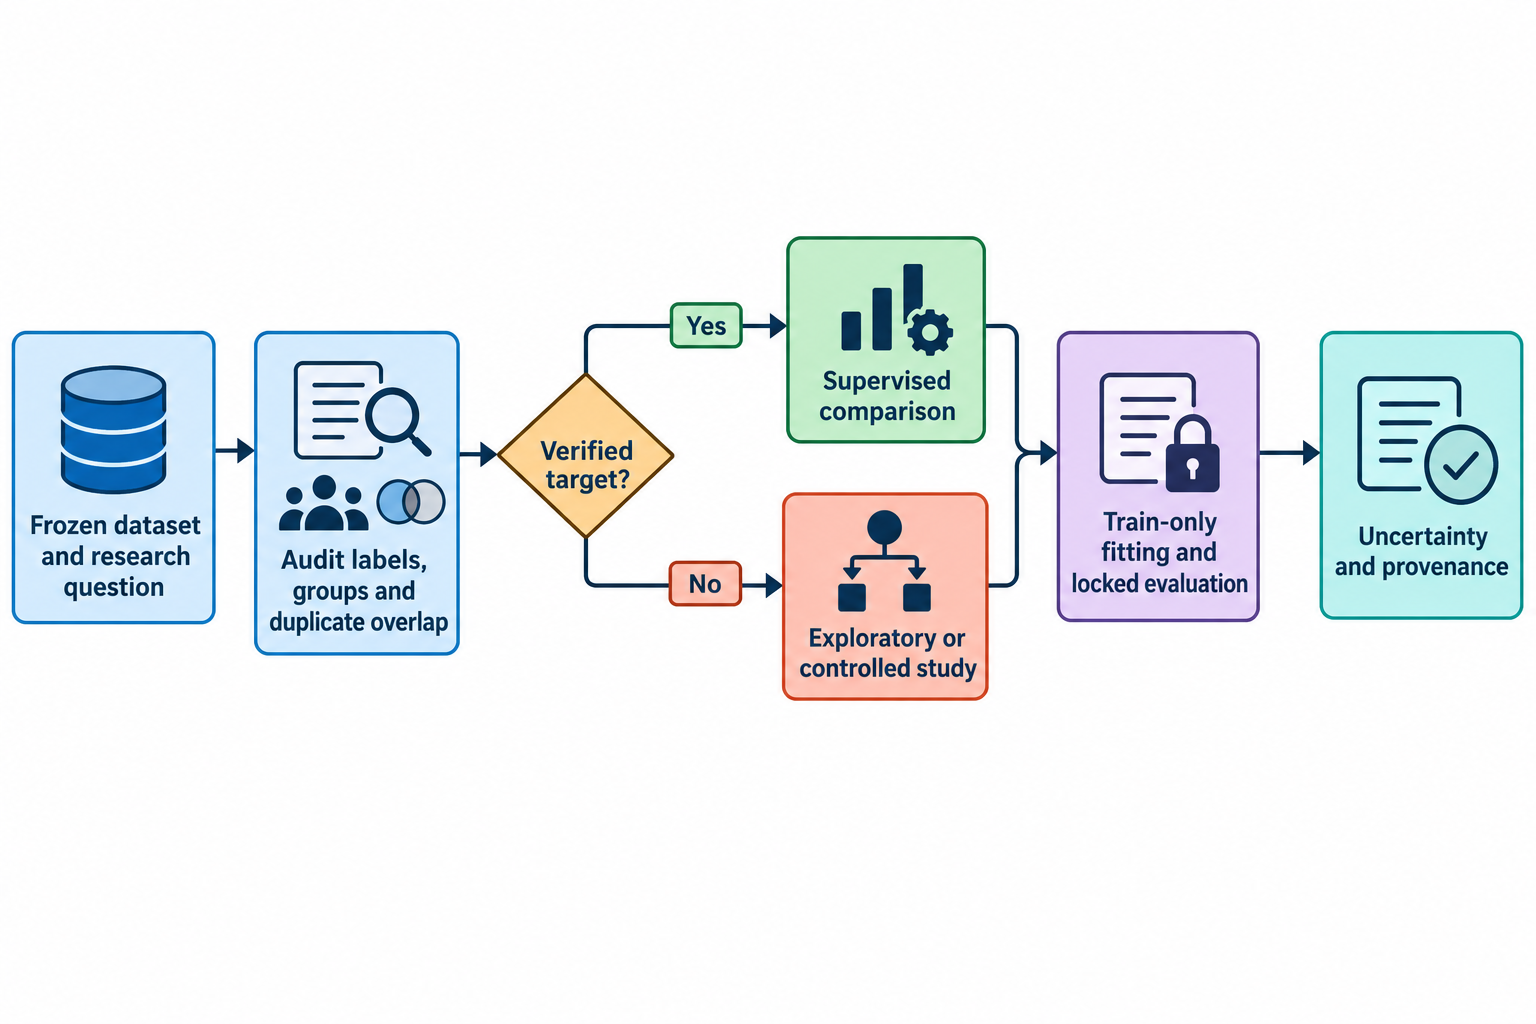
\includegraphics[width=\linewidth,trim={0bp 303bp 0bp 216bp},clip]{images/figure-06.png}\caption{Evidence quality determines which evaluation claims are supportable.}
\end{figure}
Use group-based splits when records share a description, flow, trace, entity or scenario template. Keep related versions and inverse graph facts on the same side of the split. Record exclusions and split identifiers before tuning. Fit transformations only on training data [8].

Use MITRE ATT\&CK for ICS as a vocabulary for analyst-reviewed mappings [7]. A technique association does not itself establish that an attack occurred. NIST CSF 2.0 can organize research outcomes; this dataset does not establish compliance [6].

\clearpage\section{Inventory: segmentation and exposure}
\textbf{Research area.} Asset-centric exposure analysis\newline \textbf{Problem statement.} Incomplete knowledge of communication boundaries complicates the allocation of scarce monitoring resources.

\textbf{Research question.} Can a graph-aware monitoring policy cover important cross-zone flows more efficiently than a simple priority rule?

\textbf{Materials and suitability.} Use Dataflows.csv with assets-Master.csv, ZONES.csv and zones\_conduits.csv. Treat the separate 53-record component inventory as a source requiring explicit mapping. Direct support for structural comparisons; measured intrusion likelihood and operational disruption require additional evidence.

\textbf{Experimental design.} Check asset/zone keys and join coverage; retain unmatched rows in an audit. Construct a directed asset-flow graph. Declare protocol/port and zone rules. Compare policies under equal sensor or intervention budgets.

\begin{figure}[H]\centering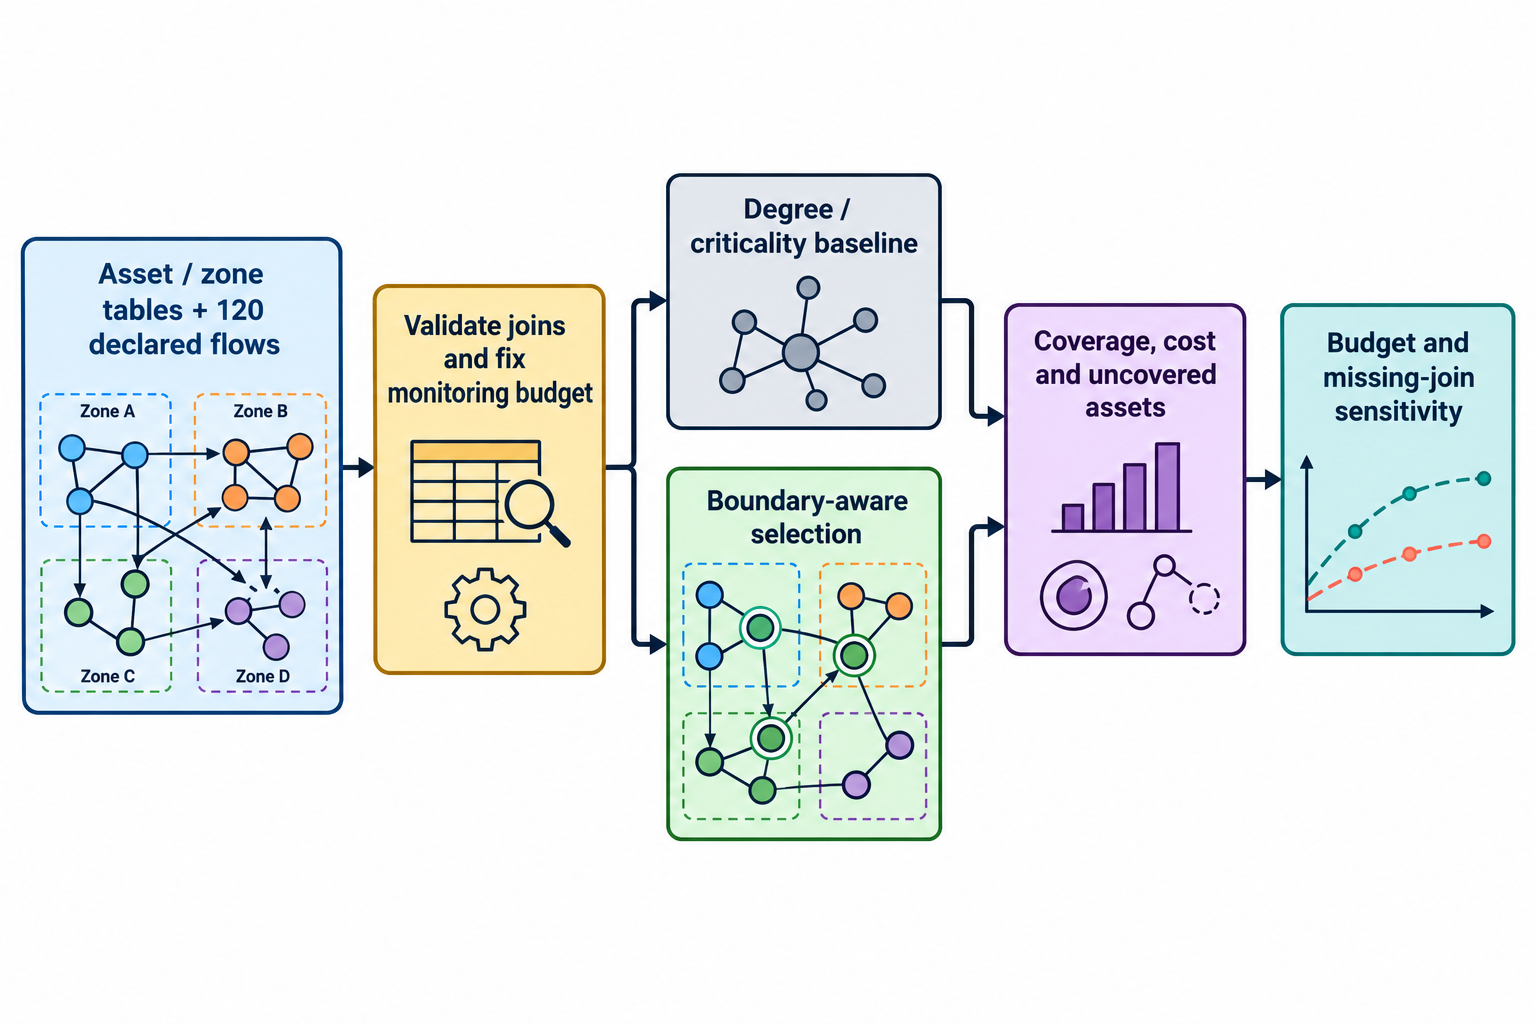
\includegraphics[width=\linewidth,trim={1bp 163bp 0bp 153bp},clip]{images/figure-07.png}\caption{A shared topology and budget enable a fair monitoring comparison. Network and curve icons are schematic, not the released topology or measured results.}
\end{figure}
\textbf{Interpretation and limitations.} Give cross-zone flow coverage, weighted coverage, selected locations and sensitivity to criticality weights. Reachability reflects declared connectivity, not proven exploitability. Removed identities and addresses cannot support deployment-specific claims.

\clearpage\section{Knowledge graph: inference and prioritization}
\textbf{Research area.} Explainable threat intelligence and graph learning\newline \textbf{Problem statement.} A plausible association between a weakness, product and technique may be unsupported or produced by leakage between training and evaluation graphs.

\textbf{Research question.} Does a typed graph method recover held-out relations better than a relation-frequency baseline?

\textbf{Materials and suitability.} Use node and edge CSV/CSV.GZ files with metadata/graph\_node\_keys.json and graph\_relation\_rules.json. The release contains 291,577 CVE rows across 15 shards. Direct support for typed structural inference; temporal forecasting requires dated snapshots and verified future outcomes.

\textbf{Experimental design.} Select one relation and a transductive or entity-disjoint task. Split before creating inverse edges, embeddings or derived features. Remove held-out facts and equivalent inverse/derived facts from training. Use type-correct candidates; document negative sampling.

\begin{figure}[H]\centering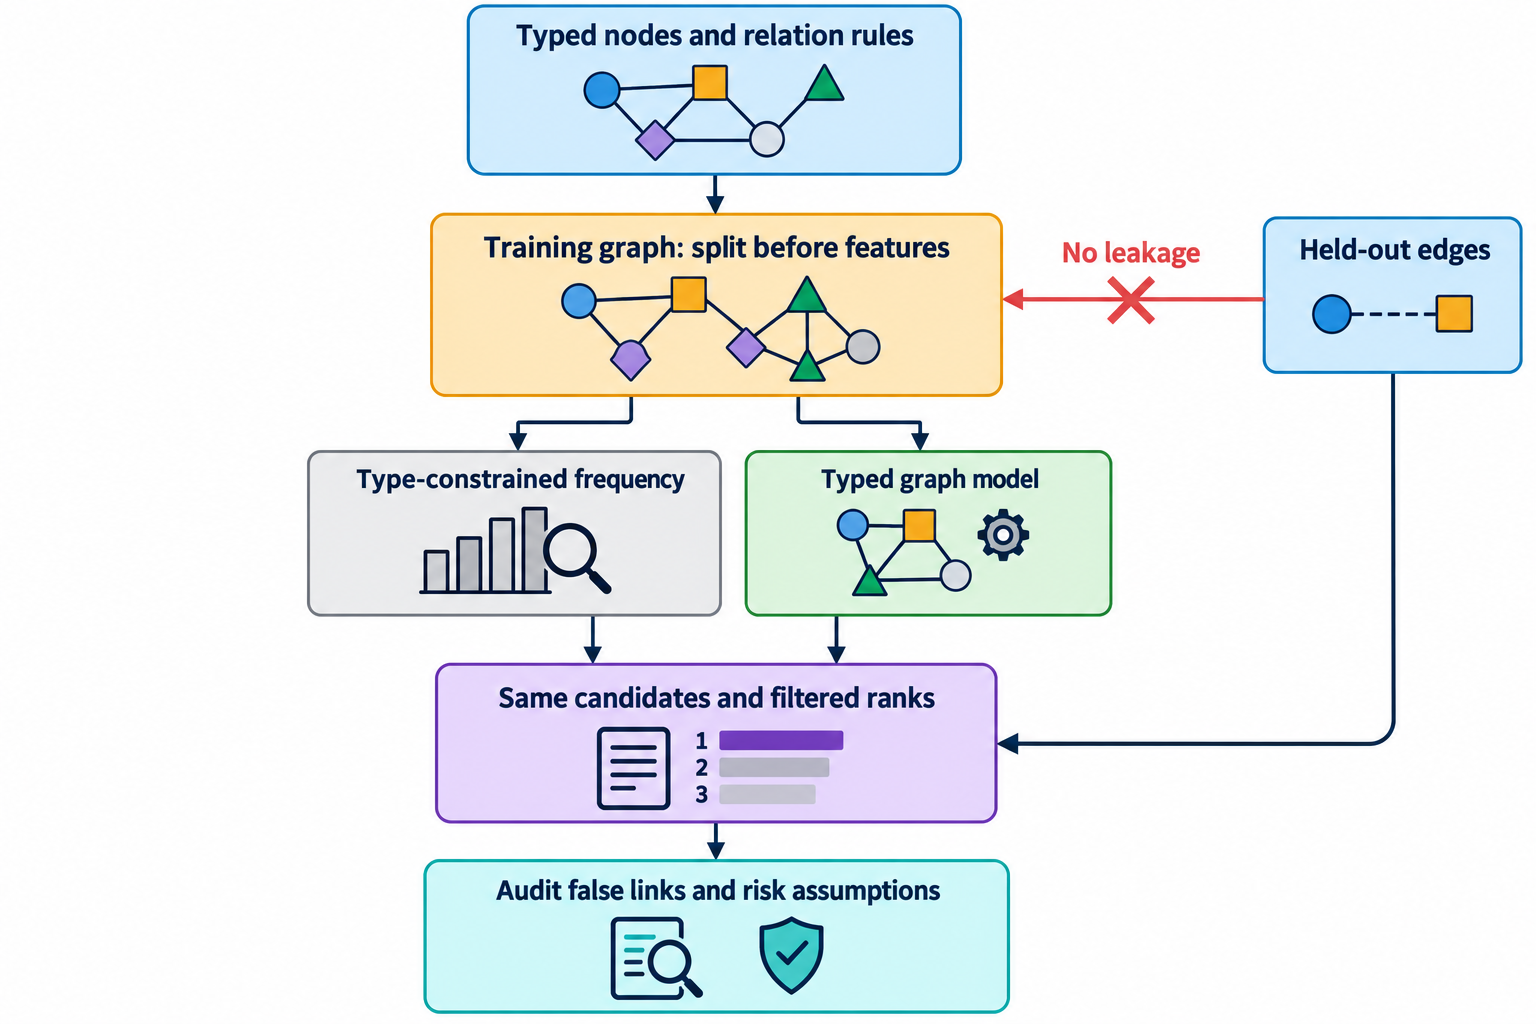
\includegraphics[width=\linewidth,trim={287bp 0bp 0bp 0bp},clip]{images/figure-08.png}\caption{Split construction precedes graph feature generation.}
\end{figure}
\textbf{Interpretation and limitations.} Report MRR and Hits@k with candidate counts, or precision/recall on a defined labeled task. Unknown edges are not verified negatives. Zero unmatched endpoints confirms structure only. CVSS/EPSS/KEV attributes are historical snapshots; they are not current risk advice. The graph lacks a full narrative corpus.

\clearpage\section{CTI benchmarks: grounded answers}
\textbf{Research area.} Evidence-grounded LLM security analytics\newline \textbf{Problem statement.} Fluent threat explanations may include incorrect identifiers or claims that are not entailed by retrieved evidence.

\textbf{Research question.} Does graph grounding improve technique or weakness mapping over the same model without retrieval?

\textbf{Materials and suitability.} Use 60 CTI-ATE, 996 CTI-RCM and 991 CTI-RCM-2021 records. GT is an upstream reference label. CTIBench is external work by Alam et al. [5], not authored by this repository maintainer. Direct support for reference-label mapping; citation faithfulness requires a separately adjudicated evidence set.

\textbf{Experimental design.} Use metadata/benchmark\_split\_groups.csv to keep related descriptions together across files. Hide GT and any direct answer-bearing path from the model input and retrieval index. Freeze prompts and retrieval budget. Normalize output to declared identifier sets; score abstentions explicitly.

\begin{figure}[H]\centering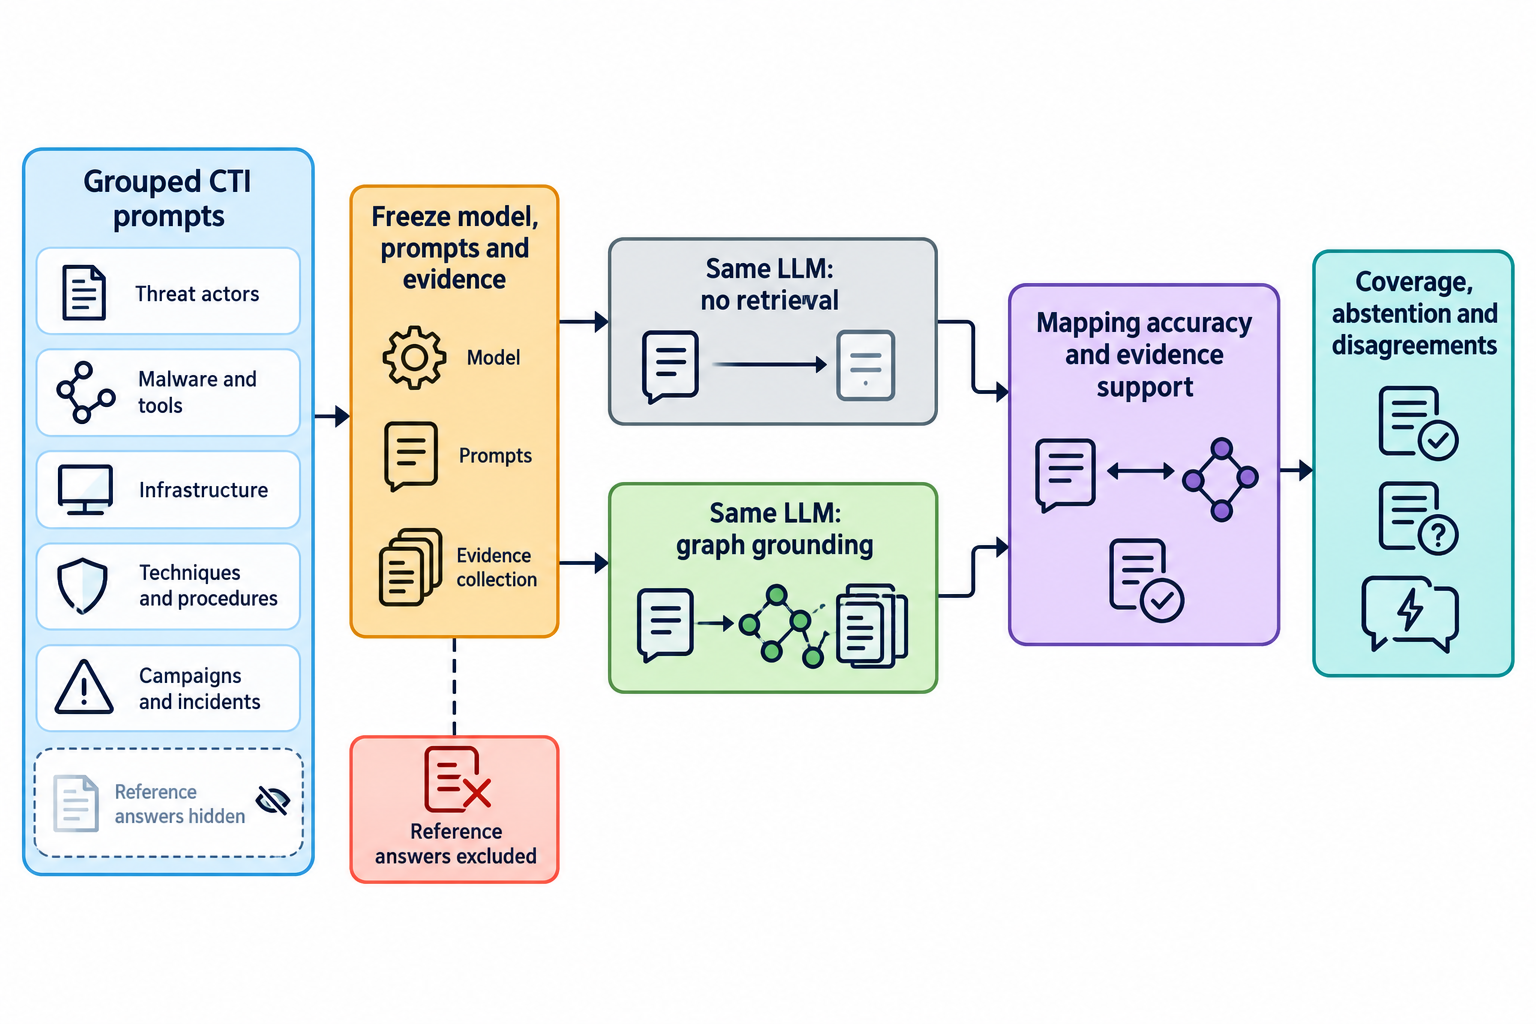
\includegraphics[width=\linewidth,trim={2bp 120bp 1bp 127bp},clip]{images/figure-09.png}\caption{Retrieval gains must be measured independently from answer leakage. CTI category icons illustrate the analytical setting, not an inventory of released benchmark labels.}
\end{figure}
\textbf{Interpretation and limitations.} Report exact-set match and micro/macro label precision, recall and F1 as appropriate to the GT representation. Distinguish parsing failures, wrong mappings and unsupported claims. Thirteen records from five conflicting-description groups were excluded during release preparation. Evaluate retained labels rather than assuming universal correctness. CTIBench terms include noncommercial/share-alike conditions.

\clearpage\section{Training pairs: query generation}
\textbf{Research area.} Domain adaptation for security query generation\newline \textbf{Problem statement.} A model may memorize query templates while failing to generate semantically correct queries for unseen analytical tasks.

\textbf{Research question.} Can instruction tuning improve schema-valid, semantically correct query generation on unseen query families?

\textbf{Materials and suitability.} fine\_tuning.json contains 358 unique instruction/output pairs after removal of 129 exact duplicates. These are development examples, not an official held-out benchmark. Conditional support: researchers must construct a disjoint evaluation set and validate query semantics.

\textbf{Experimental design.} Group near-duplicate instructions and query templates. Create train/dev/test groups and publish IDs. Reserve the test set before prompt engineering or adaptation. Compare a fixed base model with the adapted model on the same held-out prompts. Validate queries in a read-only sandbox if execution is part of the task.

\begin{figure}[H]\centering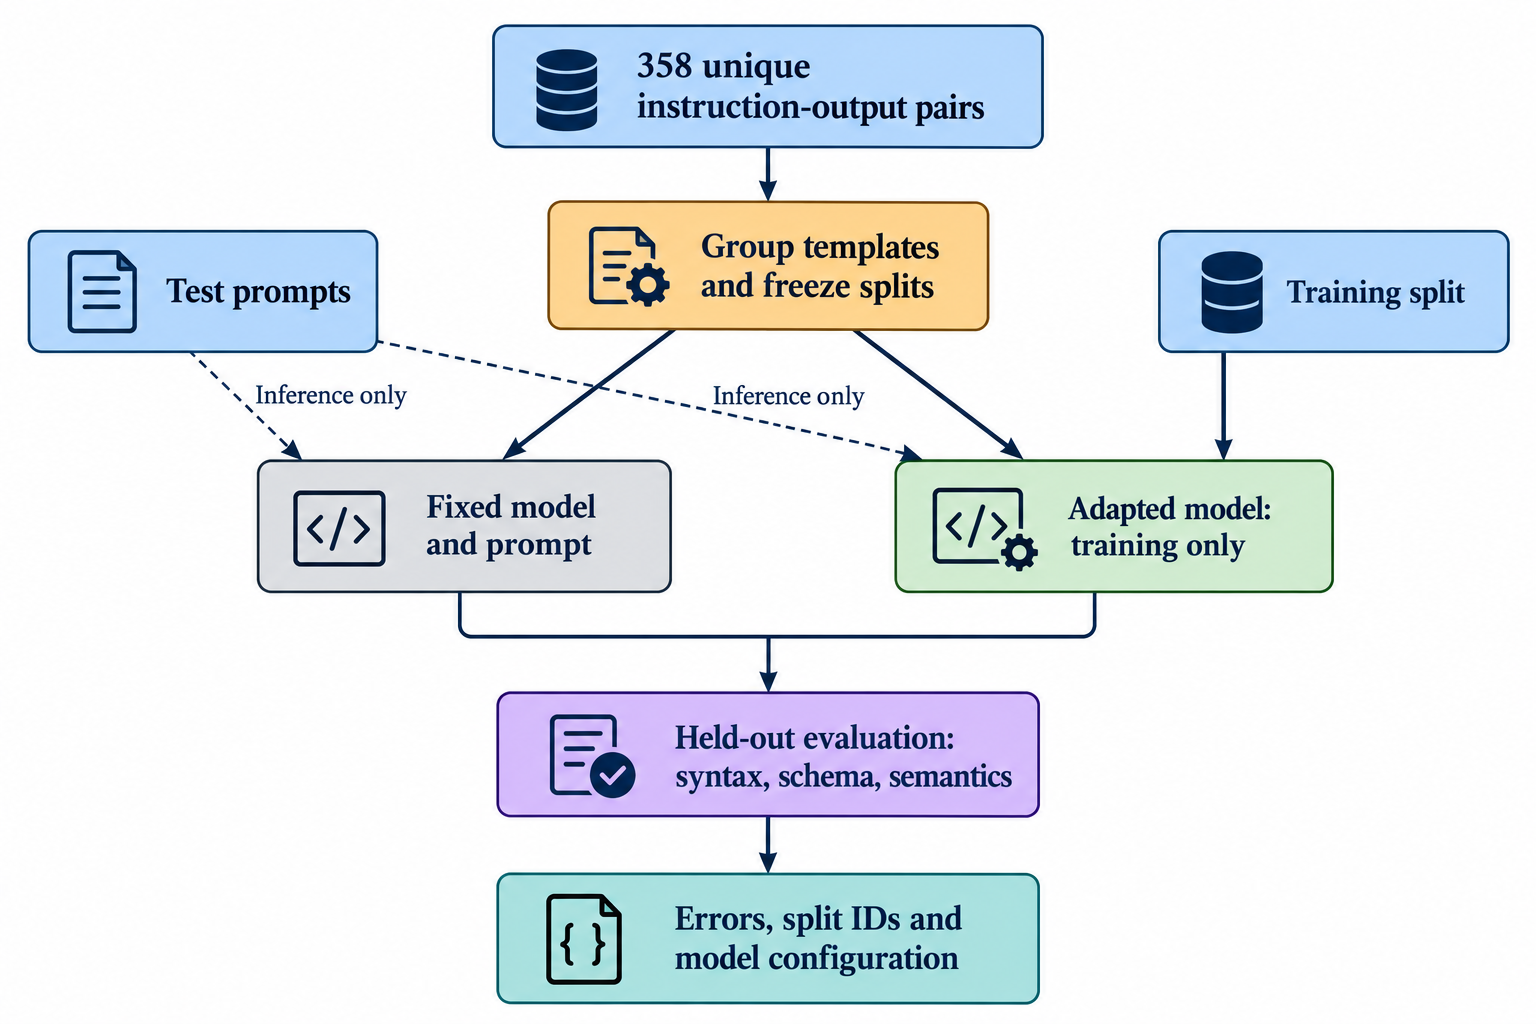
\includegraphics[width=\linewidth,trim={7bp 0bp 6bp 4bp},clip]{images/figure-10.png}\caption{Template separation reduces memorization-based evaluation.}
\end{figure}
\textbf{Interpretation and limitations.} Report syntactic validity, schema validity, execution success and semantic correctness separately. Textual exact match alone may reject equivalent queries. The release does not supply a ready-made hosted database or tuning pipeline. State any external examples, compute budget and model license; test contamination remains a limitation.

\clearpage\section{Synthetic data: controlled anomaly studies}
\textbf{Research area.} Robust detection under controlled perturbations\newline \textbf{Problem statement.} A detector can learn generation artifacts instead of behavior relevant to an intrusion or operational anomaly.

\textbf{Research question.} How robust is an anomaly detector to documented timing or volume perturbations under different protocols?

\textbf{Materials and suitability.} Use 9,880 generated protocol rows and 340 attackability rows. Protocols include OPC UA, Modbus TCP, MQTT/MQTTS, HTTPS, SSH, RDP, S7comm and EtherNet/IP. Suitable for controlled algorithm comparison; field detection claims require independently labeled operational incidents.

\textbf{Experimental design.} Inspect protocol-specific fields before harmonizing. Split by flow or generation/scenario group where supported. Add perturbations to a derived copy with a recorded seed and explicit injection labels. Keep training and test generation groups disjoint. Compare equal-threshold-budget methods.

\begin{figure}[H]\centering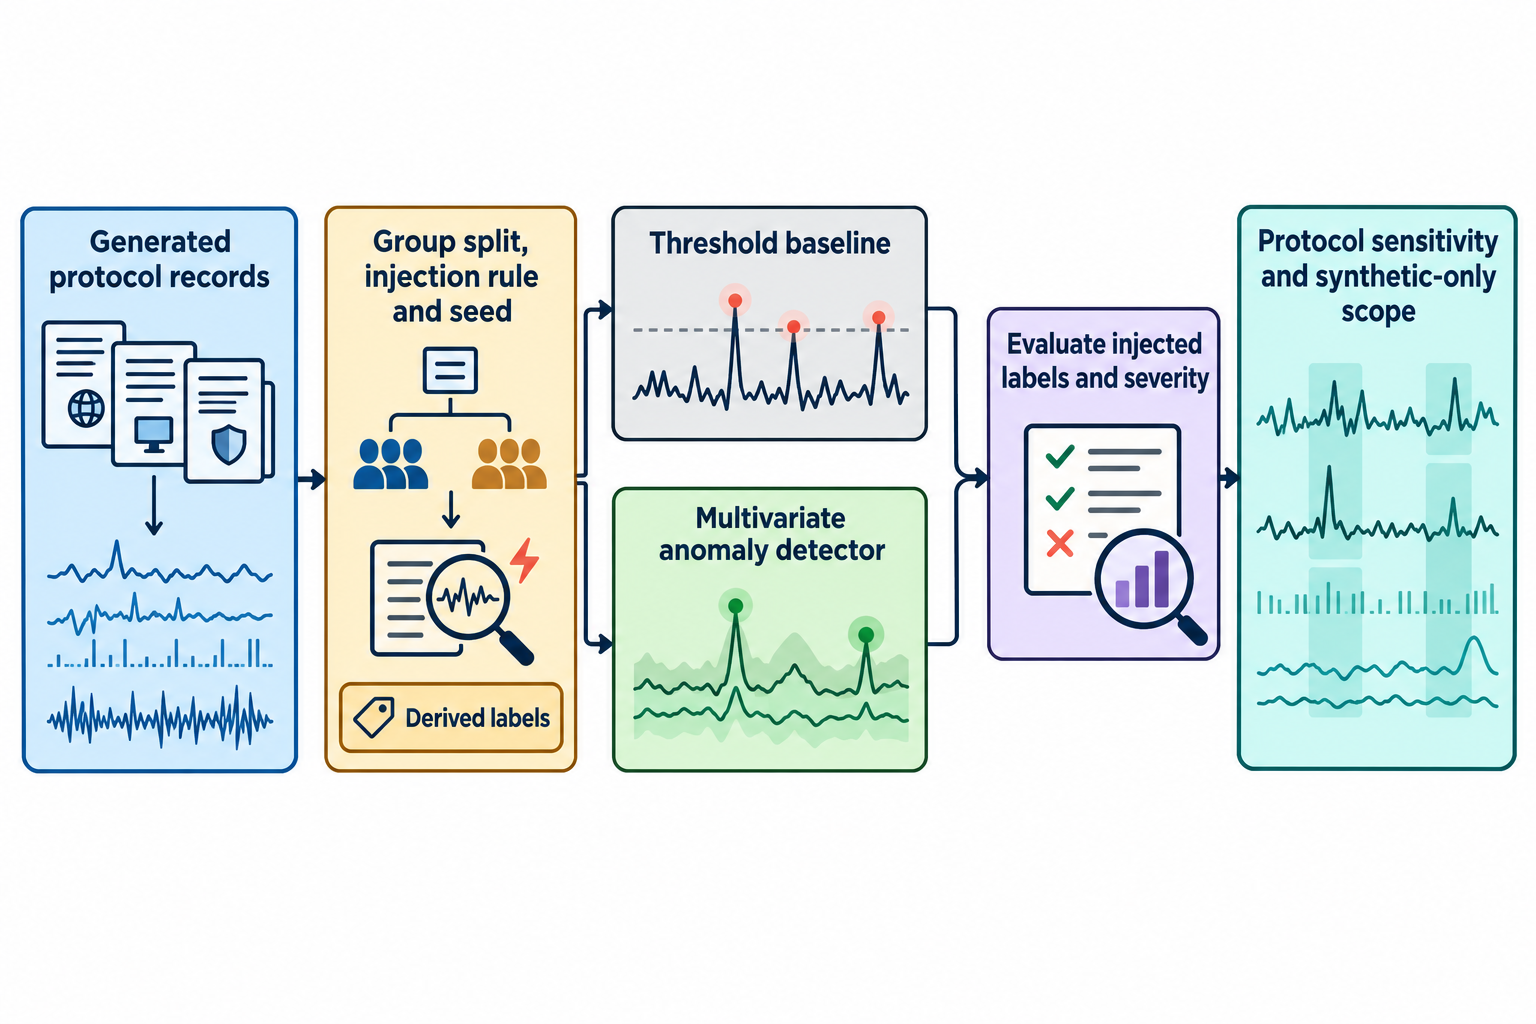
\includegraphics[width=\linewidth,trim={0bp 230bp 0bp 185bp},clip]{images/figure-11.png}\caption{Labels introduced by the experiment stay separate from released values.}
\end{figure}
\textbf{Interpretation and limitations.} Give precision/recall, PR-AUC and false alarms per declared unit for the controlled task. Status/result fields are not universal malicious labels. ATTACKABLE controlStrength, pExploit, attackCost\_min and riskWeight are synthetic assumptions, not empirical compromise outcomes. Test whether a model merely reconstructs the formula used to create its target.

\clearpage\section{Operational traces: sequence research}
\textbf{Research area.} Behavioral monitoring and sequence modelling\newline \textbf{Problem statement.} Unusual sequences can reflect legitimate operating modes, incomplete observations or faults as well as malicious activity.

\textbf{Research question.} Can a sequence model identify unusual transitions more consistently than a local transition-frequency baseline?

\textbf{Materials and suitability.} event\_features.jsonl.gz contains 14,124 records in 27 traces. Fields include trace\_id, record\_index, relative\_seconds, event\_class, signal\_id, value, previous\_value and ok. Suitable for exploratory sequence analysis; attack classification is conditional on new, verified labels.

\textbf{Experimental design.} Order within each trace using record\_index and relative time; inspect missing or repeated times. Split whole traces before creating windows. Fit encoders and thresholds on training traces only. If no independent attack labels exist, use descriptive anomaly analysis or separately labeled controlled perturbations.

\begin{figure}[H]\centering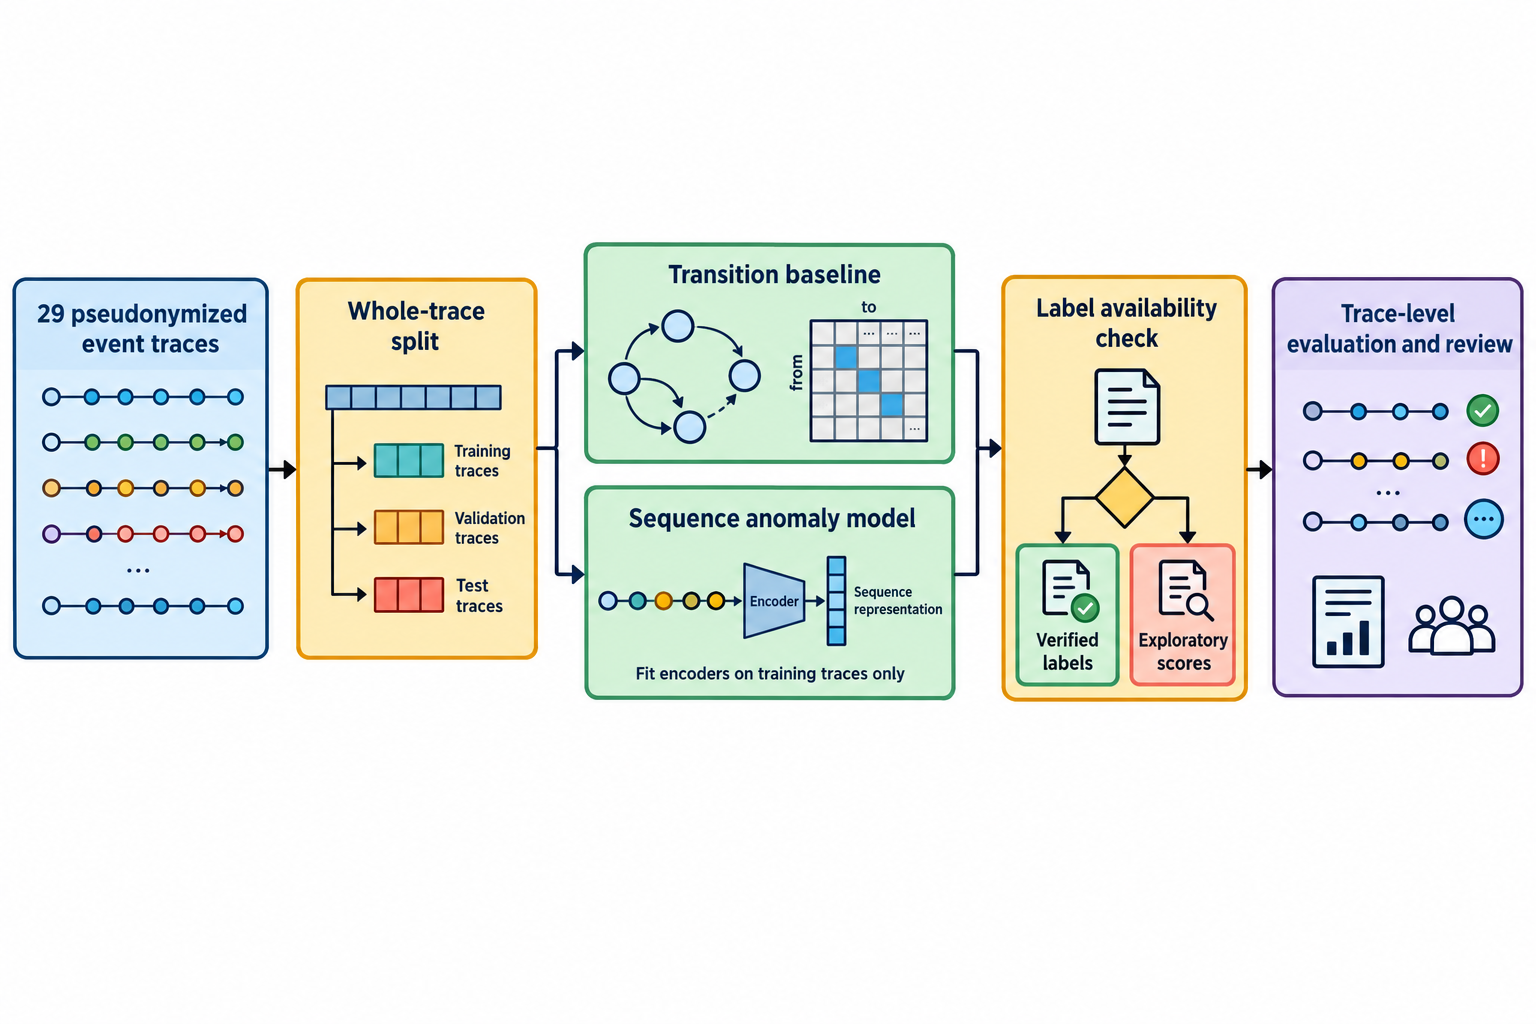
\includegraphics[width=\linewidth,trim={0bp 302bp 0bp 222bp},clip]{images/figure-12.png}\caption{Trace boundaries and label availability constrain inference.}
\end{figure}
\textbf{Interpretation and limitations.} Report unusual-transition rates and review agreement for exploratory studies; use attack metrics only with justified labels. The ok field is not an attack label. Relative clocks are per trace. String values are state\_ pseudonyms; units and original signal semantics may be unavailable. Do not infer physical meaning or align cross-trace clocks without evidence.

\clearpage\section{Agent scenarios: governed decisions}
\textbf{Research area.} Assurance of agentic security workflows\newline \textbf{Problem statement.} An AI agent may select nonexistent tools, exceed a risk condition or continue after a required stop.

\textbf{Research question.} Does a policy guard reduce invalid tool selections and missed stop conditions relative to an unguarded decision policy?

\textbf{Materials and suitability.} Use 400 expected cases across 20 JSON scenarios. Each provides inputs and expected outputs/final decisions. These fixtures are distinct from the historical twin replay suites. Direct support for fixture-based policy evaluation; live tool safety and mission success are outside the fixture evidence.

\textbf{Experimental design.} Build a local fixture evaluator that reads tests and records actual outputs. Keep expected fields out of model prompts. Group by scenario family for held-out testing where feasible. Route proposals through tool-catalog, risk and stop checks before any simulated execution. Use deterministic mock tools for comparison.

\begin{figure}[H]\centering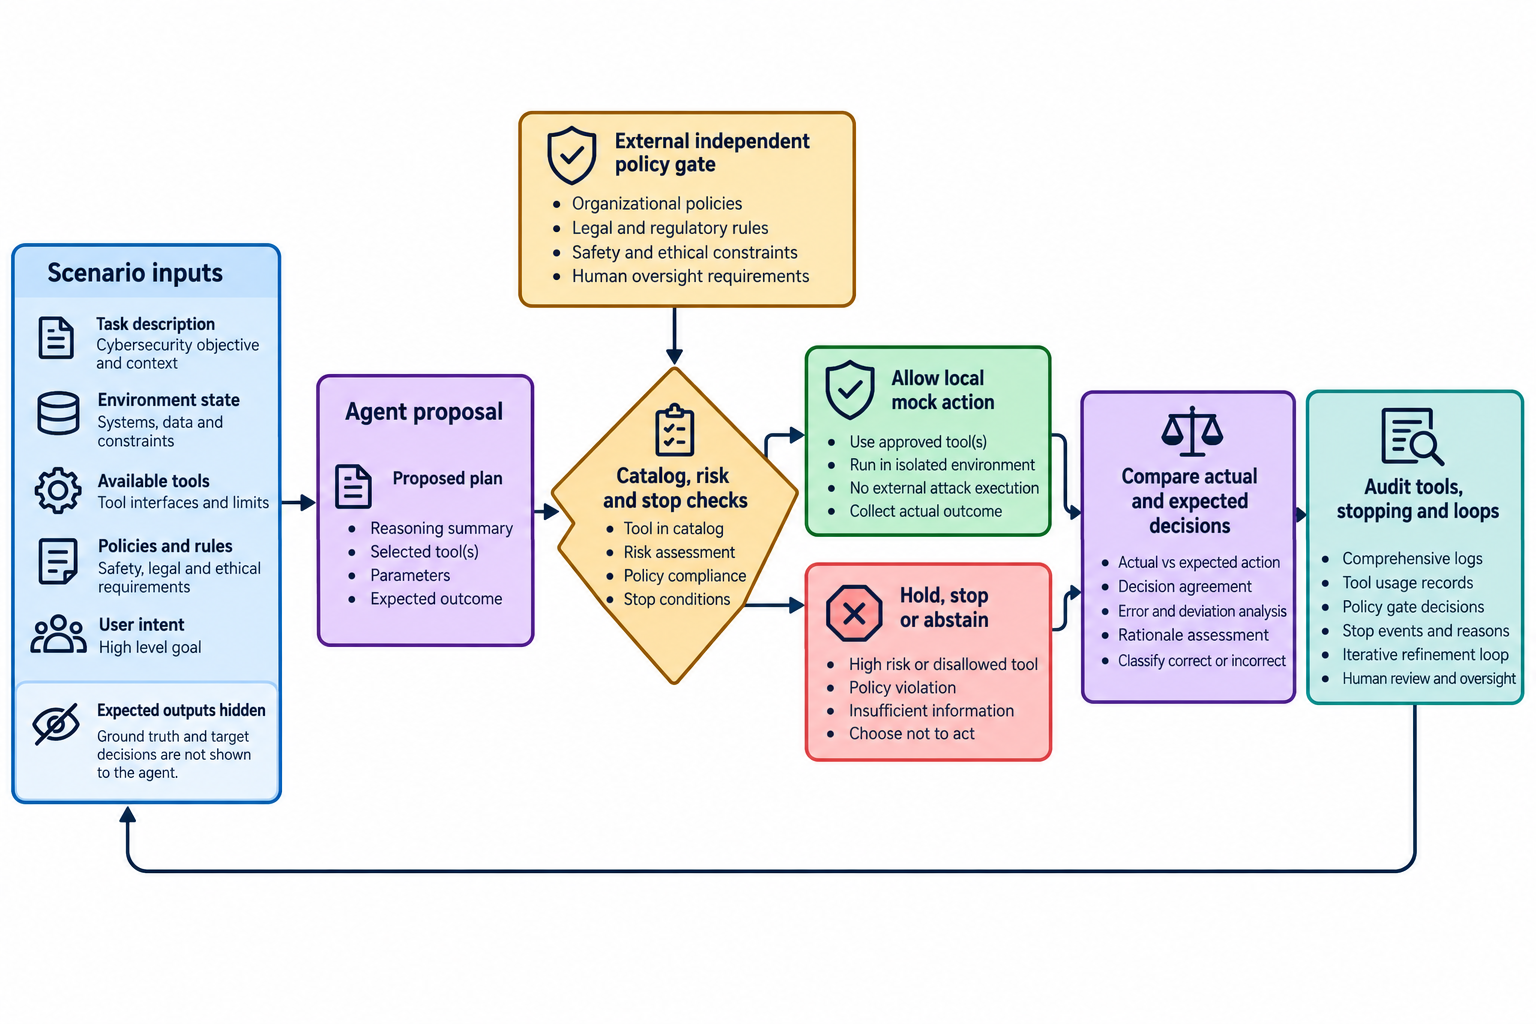
\includegraphics[width=\linewidth,trim={0bp 131bp 0bp 91bp},clip]{images/figure-13.png}\caption{The decision gate produces auditable allow/hold outcomes. Additional governance controls illustrate a proposed evaluator; they are not all encoded in the released fixtures.}
\end{figure}
\textbf{Interpretation and limitations.} Report case-level agreement, unsafe-decision rate, stop-condition recall, invalid-tool rate and bounded termination. Specify denominators and oracle limitations. Relevant fixtures cover unavailable tools, hallucinated tools, risk thresholds, loop guards and simulation-only eligibility. Expected outputs are policy references, not evidence of live attacks or operational safety certification.

\clearpage\section{Integrated study: evidence to review}
\textbf{Research area.} Human-centered evidence fusion\newline \textbf{Problem statement.} Combining incompatible identities or clocks can create convincing but false cross-source explanations.

\textbf{Research question.} Can traceable evidence improve analyst prioritization compared with an inventory-only ranking?

\textbf{Materials and suitability.} Combine only demonstrably compatible inventory keys, graph relations and event identifiers. Different sources may not share identities or clocks. Conditional support: only explicitly validated identity and temporal mappings justify integrated analyses.

\textbf{Experimental design.} Create a mapping table with source keys, mapping rationale and confidence. Measure join coverage and unresolved records before fusion. Require supported joins for each evidence chain; retain unresolved records for review rather than guessing. Compare the same analyst tasks and time budget.

\begin{figure}[H]\centering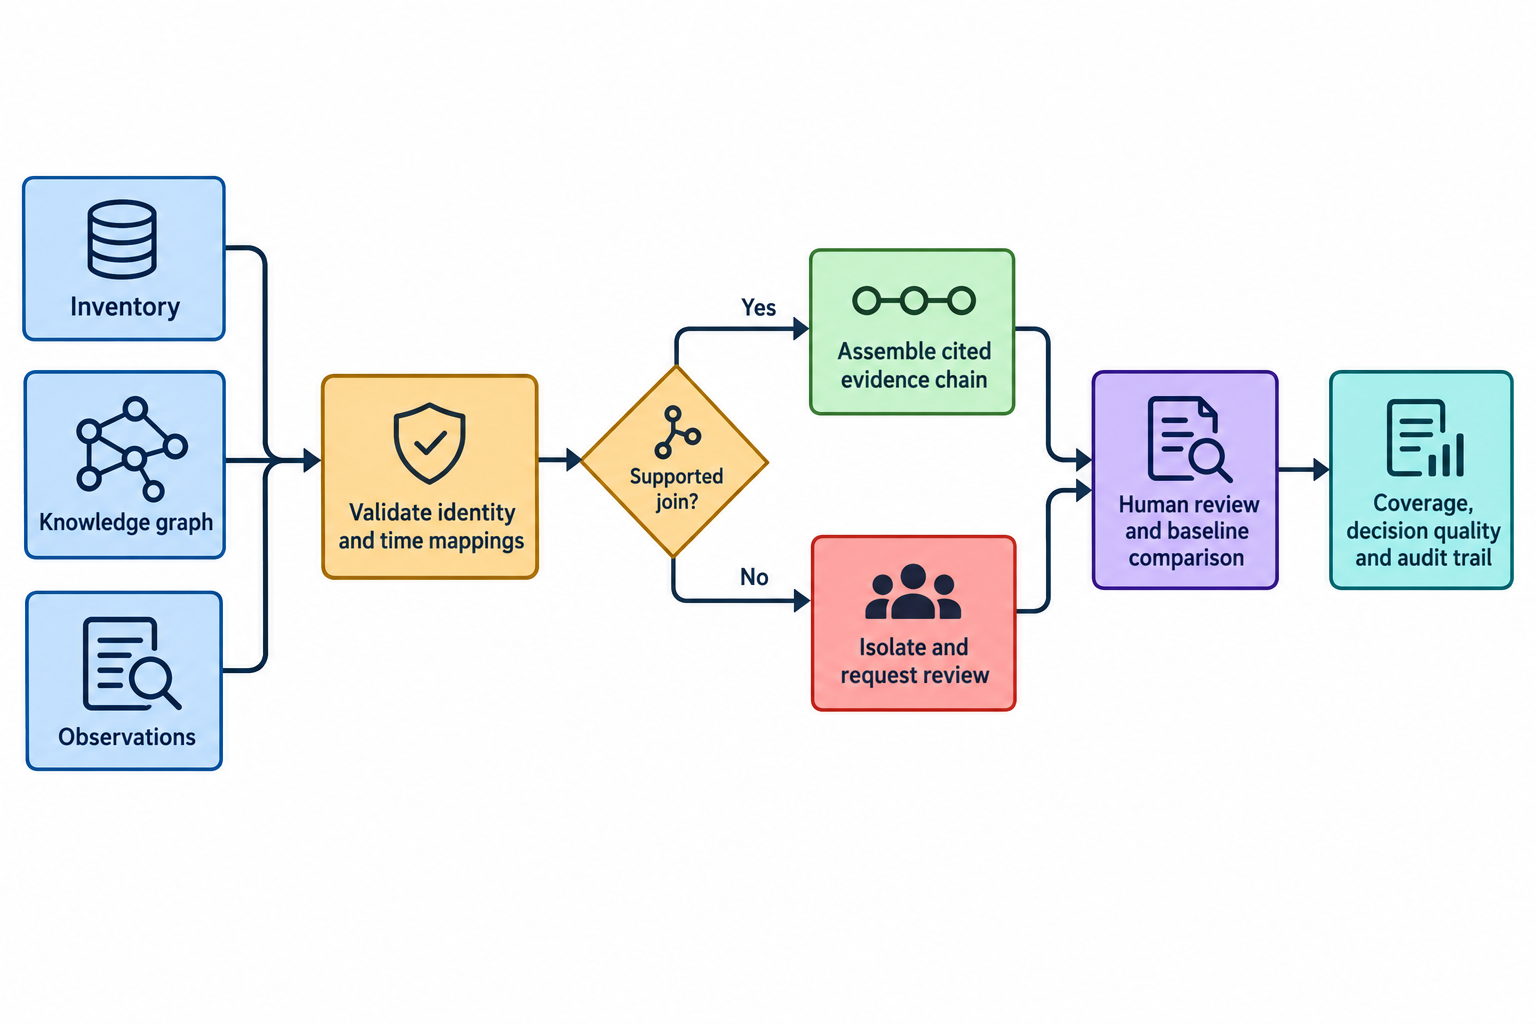
\includegraphics[width=\linewidth,trim={2bp 233bp 2bp 156bp},clip]{images/figure-14.png}\caption{Evidence joins are an eligibility gate, not an assumption.}
\end{figure}
\textbf{Interpretation and limitations.} Report supported-join coverage, unsupported-claim rate, analyst agreement and review time with the study protocol. Blind reviewers to method where practical. Do not interpret a connected path as a confirmed attack chain. Explain how pseudonymization and missing semantics affect causal interpretation.

\clearpage\section{Metrics, uncertainty and fair comparisons}
\begingroup\small\setlength{\tabcolsep}{5pt}\renewcommand{\arraystretch}{1.22}
\begin{tabularx}{\linewidth}{>{\raggedright\arraybackslash}X>{\raggedright\arraybackslash}X>{\raggedright\arraybackslash}X}
\toprule
\textbf{Task} & \textbf{Primary measures} & \textbf{Essential denominator / caveat}\\
\midrule
Label mapping & Exact set match; micro/macro F1 & All eligible prompts; disclose parse failures and abstentions\\
Graph ranking & MRR; Hits@k & Candidate set size; filtered-known-fact rule; unknown negatives\\
Anomaly detection & PR-AUC; precision/recall; false alarms & Verified or injected labels; alarms per trace/time unit\\
Inventory optimization & Coverage; cost; uncovered critical flows & Fixed budget and declared weights; unmatched joins\\
Query generation & Syntax, schema and semantic validity & All test prompts; distinguish equivalent queries\\
Agent decisions & Agreement; invalid-tool and stop-failure rates & All eligible cases; independent failures may overlap\\
\bottomrule\end{tabularx}\endgroup\par\medskip
Define TP, FP and FN for the chosen positive unit. Precision = TP/(TP+FP); recall = TP/(TP+FN); F1 = 2PR/(P+R). State how zero denominators are handled. Accuracy alone can obscure rare-event failure.

Use identical splits, candidate sets, prompts and resource budgets across methods. Report multiple seeds for stochastic training. Bootstrap or summarize at the independent unit, such as trace, description group or scenario family; row-level resampling can understate uncertainty.

Use ablations that answer a question: remove graph evidence, remove policy guards, or replace a learned detector with a simple threshold. Report confidence intervals with method and sample size, practical effect size, failure cases and computational cost. Small numbers of independent groups limit generalization.

\clearpage\section{Replay the reference experiments}
The release includes curated historical code under code/twin\_reference and an offline orchestration script. Replaying this code checks reproducibility of its included fixtures. It does not train every proposed model in this guide or reproduce every paper claim.

\begin{Verbatim}[fontsize=\footnotesize,breaklines=true,frame=single,rulecolor=\color{rulegray},framesep=8pt]
python -m venv .venv
# Activate this environment using your platform convention.
python -m pip install -r code/requirements-replay.txt
python scripts/replay_offline.py --help
python scripts/replay_offline.py --source-root . --output replay_output
\end{Verbatim}
Use a clean environment and retain the installed package versions. Inspect scripts/replay\_offline.py and docs/VALIDATION.md for the dependency-directory option and current execution behavior. Keep replay\_output outside the published source manifest.

\subsection*{Interpret the recorded baseline correctly}
validation/replay\_summary.json records the prior release replay: 24 suites, 285 tests and 10 deterministic experiments. These are recorded validation results for the curated code, not a fresh model benchmark or a pass count for the 400 agent-scenario cases. A new run must report its own result and environment.

\subsection*{What to retain from a new run}
\begin{itemize}
\item Exact repository commit, input checksums, command line and dependency versions.
\item Per-suite exit status, test totals, experiment outputs and failure logs.
\item Any local patches, model/provider configuration, seeds and elapsed time.
\item A comparison of expected versus actual outputs; explain deviations without overwriting the reference result.
\end{itemize}
Offline fixtures do not require physical equipment, model weights, a hosted graph database or live network actions. If a separate study introduces those components, describe them as additional experimental infrastructure and report the authorization and isolation appropriate to that study.

\clearpage\section{Prepare a reusable research package}
\subsection*{Minimal experiment manifest - fill in actual values}
\begin{Verbatim}[fontsize=\footnotesize,breaklines=true,frame=single,rulecolor=\color{rulegray},framesep=8pt]
study_id: your-study-id
dataset_commit: FULL_COMMIT_SHA
input_paths: [SELECTED_RELEASE_FILES]
input_sha256_manifest: metadata/checksums.csv
question: PREDECLARED_QUESTION
unit_of_analysis: trace_or_group_or_entity
label_source: reference_or_adjudicated_or_injected_or_none
split_ids: path/to/frozen_split_ids.json
seed: YOUR_SEED
baseline: VERSION_AND_CONFIGURATION
method: VERSION_AND_CONFIGURATION
fit_scope: training_only
primary_metric: METRIC_AND_DENOMINATOR
uncertainty: METHOD_AND_RESAMPLING_UNIT
outputs: path/to/results
exclusions_and_limitations: path/to/audit.md
\end{Verbatim}
\subsection*{Before submission or release}
State the cybersecurity question and threat assumptions; describe the exact subset and independent sample count; publish group splits and exclusions; separate observations from synthetic or expected values; include baselines and ablations; report all eligible outcomes, uncertainty and failures; and disclose external enrichment, model versions and compute.

Cite this dataset using CITATION.cff and cite the relevant original works [1-5]. Read LICENSE, LICENSE-CODE, THIRD\_PARTY\_NOTICES.md and metadata/licenses.csv: the compilation, code and third-party subsets have different terms. CTIBench is CC BY-NC-SA 4.0; a top-level badge does not override subset conditions.

Keep pseudonymized identifiers as released. Do not restore private identities or publish unreviewed source material. Share derived labels with their creation protocol and clear provenance. A public dataset paper should describe collection, curation, schema, permitted uses, quality checks and limitations separately from a method paper's performance claims.

\clearpage\section{Articles and methodological references}
Article attribution and publication status follow docs/RELATED\_PUBLICATIONS.md. A related article is context for a research theme, not proof that this curated subset reproduces its results.

\textbf{[1] BRIDG-ICS: AI-grounded knowledge graphs for intelligent threat analytics in Industry 5.0 cyber-physical systems}\newline Nandiya et al. (2026). Cybersecurity 9, article 167. Published journal article.\newline \href{https://doi.org/10.1186/s42400-026-00597-0}{https://doi.org/10.1186/s42400-026-00597-0}

\textbf{[2] NeuroGraph: An AI Graph-Driven Neuro-Symbolic Framework for Explainable Threat Reasoning in Advanced Manufacturing}\newline Nandiya et al. (2026). Preprint arXiv:2609.00604. Author reports acceptance in International Journal of Information Security; final journal DOI not supplied.\newline \href{https://arxiv.org/abs/2609.00604}{https://arxiv.org/abs/2609.00604}

\textbf{[3] A Unified Framework for Human-AI Collaboration in Security Operations Centers with Trusted Autonomy}\newline Mohsin et al. (2026). ACM Transactions on Internet Technology. Journal DOI below; preprint arXiv:2505.23397.\newline \href{https://doi.org/10.1145/3837073}{https://doi.org/10.1145/3837073}

\textbf{[4] HySecTwin: A Knowledge-Driven Digital Twin Framework Augmented with Hybrid Reasoning for Cyber-Physical Systems}\newline Holmes et al. (2026). Preprint arXiv:2605.11682. Related project: HybridSec-Digital-Twin-CSP-Modelling, ahmadspm on GitHub.\newline \href{https://arxiv.org/abs/2605.11682}{https://arxiv.org/abs/2605.11682}

\textbf{[4a] Autonomous Cyber-Physical Security Assessment in Smart Manufacturing with a Behavioural Digital Twin and Agentic AI}\newline Nandiya, Mohsin, Lohmann, Ekelhart, Sarker and Janicke (n.d.). Research manuscript.\newline \href{https://github.com/ahmadspm/industrial-cps-security-datasets/blob/main/docs/RELATED_PUBLICATIONS.md}{Related-publications record in this repository}

\textbf{[5] CTIBench: A benchmark for evaluating LLMs in cyber threat intelligence}\newline Alam, Bhusal, Nguyen and Rastogi (2024). NeurIPS 37, 50805-50825. External benchmark; not authored by the maintainer.\newline \href{https://doi.org/10.52202/079017-1607}{https://doi.org/10.52202/079017-1607}

\textbf{[6] The NIST Cybersecurity Framework (CSF) 2.0}\newline NIST (2024). CSWP 29. Outcome vocabulary for framing research; not an evaluation certificate.\newline \href{https://doi.org/10.6028/NIST.CSWP.29}{https://doi.org/10.6028/NIST.CSWP.29}

\textbf{[7] ATT\&CK for ICS matrix}\newline MITRE. Technique and tactic vocabulary.  preserve the version used for mappings.\newline \href{https://attack.mitre.org/matrices/ics/}{https://attack.mitre.org/matrices/ics/}

\textbf{[8] Common pitfalls and recommended practices}\newline scikit-learn documentation. Train/test separation and leakage prevention. \newline \href{https://scikit-learn.org/stable/common_pitfalls.html}{https://scikit-learn.org/stable/common\_pitfalls.html}



\clearpage\subsection*{Earlier foundations and related sector application}
\textbf{[15] Digital Twins and the Future of Their Use Enabling Shift Left and Shift Right Cybersecurity Operations}\newline Mohsin, A., Janicke, H., Nepal, S., and Holmes, D. (2023). In \textit{2023 5th IEEE International Conference on Trust, Privacy and Security in Intelligent Systems and Applications (TPS-ISA)}, pp. 277--286.\newline \href{https://doi.org/10.1109/TPS-ISA58951.2023.00042}{doi:10.1109/TPS-ISA58951.2023.00042}; \href{https://arxiv.org/abs/2309.13612}{September 2023 preprint}.

\textbf{[16] Explainable AI for cybersecurity automation, intelligence and trustworthiness in digital twin: Methods, taxonomy, challenges and prospects}\newline Sarker, I. H., Janicke, H., Mohsin, A., Gill, A., and Maglaras, L. (2024). \textit{ICT Express}, 10(4), 935--958.\newline \href{https://doi.org/10.1016/j.icte.2024.05.007}{doi:10.1016/j.icte.2024.05.007}.

\textbf{[17] Security risks and privacy challenges in digital twins}\newline Mohsin et al. (2026). In \textit{Foundations of Digital Twins}, pp. 239--252. Elsevier.\newline \href{https://doi.org/10.1016/B978-0-443-43896-7.00016-9}{doi:10.1016/B978-0-443-43896-7.00016-9}.

\textbf{[18] A Secure-by-Design Virtual Twin Framework for AI-Driven Threat Modeling in Railway OT Systems}\newline Neupane, N., Mohsin, A., Sarker, I. H., Sikos, L. F., and Janicke, H. (2026). KES 2026.\newline \href{https://www.researchgate.net/publication/414633139_A_Secure-by-Design_Virtual_Twin_Framework_for_AI-Driven_Threat_Modeling_in_Railway_OT_Systems}{ResearchGate record}.
